\chapter{Usar GitHub como repositorio remoto}
\href{https://github.com/}{GitHub} es un portal donde podemos crear repositorios para poder usarlo como sistema centralizado de nuestros proyectos.

Entre las característica que tiene, se pueden destacar:
\begin{itemize}
    \item Entorno gráfico para controlar el repositorio. Se puede ver el histórico del repositorio, quién ha realizado los cambios, cuándo, ramas creadas...
    \item Control de incidencias. Para poder crear “\textit{issues}” del proyecto a medida que encontremos errores.
    \item Generar documentación por proyecto en formato Wiki.
    \item Gestión de “\textit{pull requests}” para integrar cambios en la rama principal.
    \item Sistema de “acciones”, que ayudan para el sistema de “integración continua”. Con estas acciones podemos generar “\textit{releases}”, compilar el código y comprobar si hay errores, pasar tests, ... Hay mucha \href{https://docs.github.com/en/actions}{documentación} al respecto.
\end{itemize}

\section{Crear repositorio}

Una vez hemos creado una cuenta, podremos crear un nuevo repositorio en la plataforma. Al crearlo, podemos elegir distintas configuraciones:

\begin{itemize}
    \item \textbf{Nombre del repositorio}, para poder acceder a él. Es recomendable darle un nombre significativo al proyecto.
    \item \textbf{Descripción}, donde podremos indicar un poco de texto para entender de qué trata el proyecto.
    \item \textbf{Visibilidad}. Podemos hacer que el repositorio sea \textbf{público} (cualquier persona puede ver el contenido del proyecto) o \textbf{privado} (sólo nuestro usuario puede verlo).

    \item \textbf{Inicializar el proyecto con}: Podemos hacer que cuando Github inicialice el proyecto le añada ciertos ficheros:
    \begin{itemize}
        \item \textbf{README}: Fichero donde indicar de qué trata el fichero, cómo compilarlo, ...
        \item \textbf{.gitignore}: Un fichero que nos permite ignorar ficheros dentro de nuestro “área de trabajo”. Podemos elegir de una plantilla para distintos lenguajes de programación.
        \item \textbf{Licencia}: Un fichero con distintas licencias libres para nuestro proyecto.
    \end{itemize}
\end{itemize}


\begin{center}
    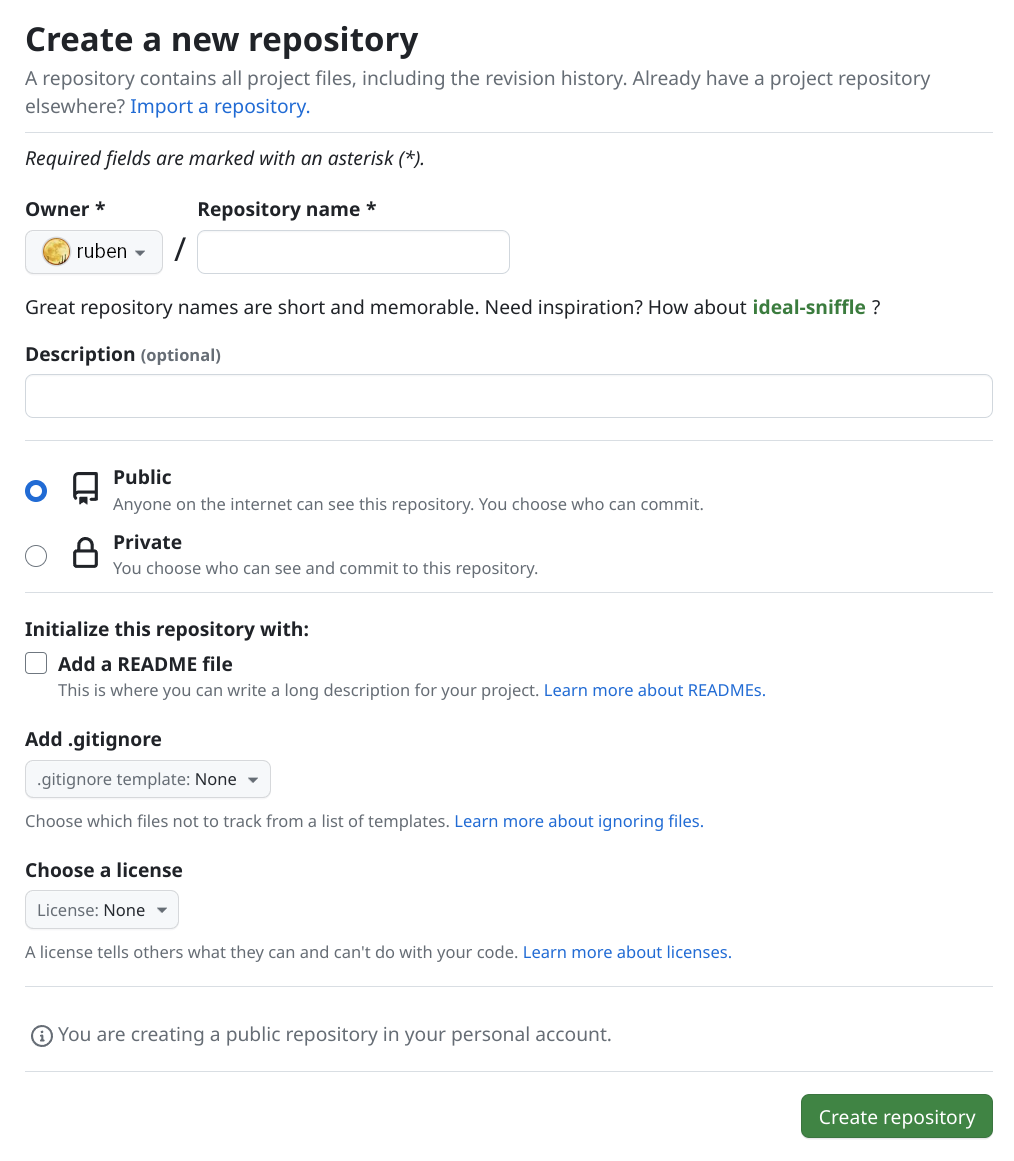
\includegraphics[frame,width=0.7\linewidth]{github-new.png}
    \captionof{figure}{Opciones al crear un nuevo repositorio en GitHub}
\end{center}

En este caso se va a crear un repositorio público llamado \textbf{pruebas}, sin ningún tipo de fichero. De esta manera “enlazaremos” el repositorio local de los pasos anteriores con este repositorio.